\documentclass{standalone}
\usepackage{amsmath}
\usepackage[dvipsnames]{xcolor}
\usepackage{tikz} 
\usetikzlibrary{arrows, decorations.markings,decorations.pathreplacing,angles,quotes}
\usepackage{microtype}
\usepackage{fourier}

\definecolor{py_blue}{rgb}{0.12156862745098039, 0.4666666666666667, 0.7058823529411765}
\definecolor{py_orange}{rgb}{1.0, 0.4980392156862745, 0.054901960784313725}
\definecolor{py_green}{rgb}{0.17254901960784313, 0.6274509803921569, 0.17254901960784313}
\definecolor{py_red}{rgb}{0.8392156862745098, 0.15294117647058825, 0.1568627450980392}
\definecolor{py_purple}{rgb}{0.5803921568627451, 0.403921568627451, 0.7411764705882353}

\begin{document}

\begin{tikzpicture}
	\node[anchor=south west,inner sep=0] (Bild) at (0,0) {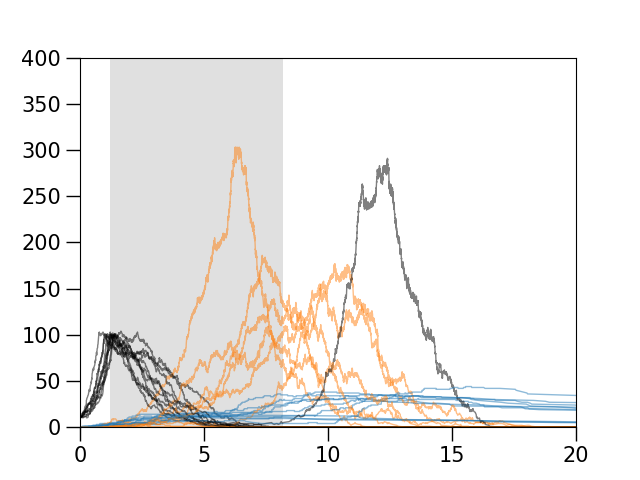
\includegraphics[scale=0.39]{low_blank}};
   		\begin{scope}[x=(Bild.south east),y=(Bild.north west)]
   			\node (B2) at ([xshift=2.75cm]Bild.east) {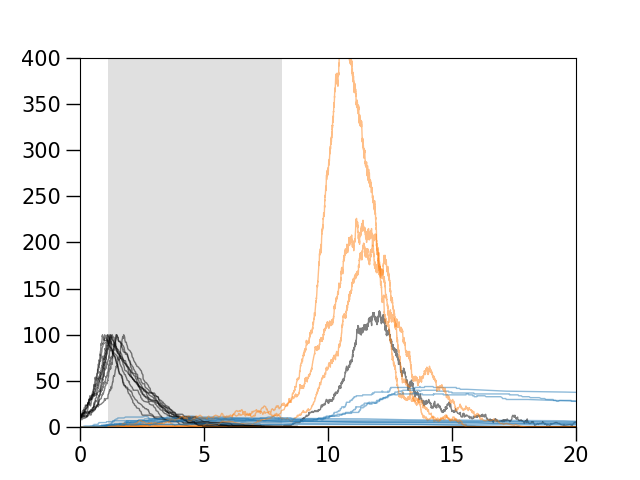
\includegraphics[scale=0.39]{inter_blank}};
   			\node (B3) at ([xshift=2.75cm]B2.east) {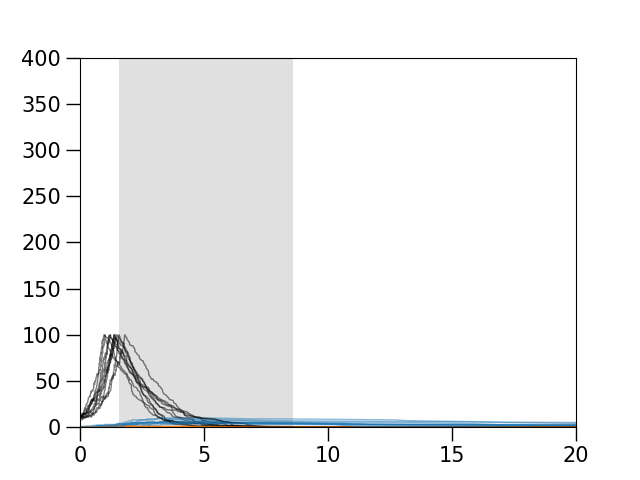
\includegraphics[scale=.39]{high_blank}};
                	
        	\node at ([yshift=-.2cm]B2.south) {\Large time in days};
        	\node[rotate=90] at ([xshift=-.4cm,yshift=-0cm]Bild.west) {\Large number of cells};
        	\node at ([yshift=-.2cm]Bild.north) {\Large $c = 0.017 = \text{mic}_S$};
        	\node at ([yshift=-.3cm]B2.north) {\Large $c=0.1 < \text{mic}_R$};
        	\node at ([yshift=-.3cm]B3.north) {\Large $c=0.2 > \text{mic}_R$};
        		
			\draw[thick,color=py_orange] (2.45,0.7) -- node[right=5pt] {\color{black} resistant} (2.5,0.7);        	
			\draw[thick,color=black] (2.45,0.8) -- node[right=5pt] {\color{black} sensitive} (2.5,0.8);    
			\draw[thick,color=py_blue] (2.45,0.6) -- node[right=5pt] {\color{black} immune} (2.5,0.6);  
			\node at (2.57,0.53) {cells};
			
			\node[right=0pt] (t1) at (1.13,0.8) {\small treatment};
			\node at (t1.south) {\small window};   
 			
    	\end{scope}
\end{tikzpicture}

\end{document}